\documentclass[a4paper,twoside]{article}

\usepackage{epsfig}
\usepackage{subcaption}
\usepackage{calc}
\usepackage{amssymb}
\usepackage{amstext}
\usepackage{amsmath}
\usepackage{amsthm}
\usepackage{multicol}
\usepackage{mathptmx}  
\usepackage{algorithm2e}
\usepackage[bottom]{footmisc}
\usepackage{SCITEPRESS}     

\begin{document}

\title{RISC-V Accelerated Processors on FPGA: Survey of Architecture and Design}

\author{
\authorname{
\text{Arjun Salunkhe$^{1}$*, Atharva Bhosale$^{1}$, Srushti Shinde$^{1}$, Sourabh Bansode$^{1}$, Kanchan Vaidya$^{2}$*}
}
\affiliation{
\sup{1}Student at Ajeenkya DY Patil School of Engineering, India
}
\affiliation{
\sup{2}Assistant Professor at Ajeenkya DY Patil School of Engineering, India
}
\email{\text{arjun.salunkhe@proton.me} \quad | \quad \text{kanchansvaidya@gmail.com}}
}

\keywords{RISC-V, FPGA, Hardware Description Language (HDL), VHDL, 32-bit processor, ISA, APU, GPU-Accelerated Computing, RISC-V APU, 5 stage pipelining, System on Chip (SoC), Open Source, Digital Logic Design, Computer Architecture, RV32I, Vortex, e-GPU}

\abstract{This survey paper reviews recent research and development efforts on Field Programmable Gate Array (FPGA) based implementations of Reduced Instruction Set Computing version Five (RISC-V) Accelerated Processing Units (APUs) that integrate CPU and GPU capabilities on a unified platform. Focused primarily on RV32I processors extended with SIMD/SIMT architectures and GPU-specialized accelerators, this work examines open-source Hardware Description Language (HDL) implementations targeting resource-efficient computing. Key topics include architectural trade-offs, programmability, and hardware-software co-design challenges. Architectures such as Vortex and e-GPU serve as case studies for RISC-V–based GPU design strategies, while open-source RISC-V CPU implementations like RV32I (e.g., RISCY) complement these efforts, providing valuable insights for APU design.}

\onecolumn \maketitle \normalsize \setcounter{footnote}{0} \vfill

\section{\uppercase{Introduction}}
\label{sec:introduction}

The RISC-V Instruction Set Architecture (ISA) is a modern, open, and modular processor design standard that offers extensibility and customization beyond proprietary ISAs. Among its foundational subsets, the 32-bit RV32I base ISA provides a simple yet solid instruction framework, making it a popular choice for lightweight embedded processors and educational FPGA projects. The open-source nature and simplicity of RV32I enable rapid development and extension for diverse applications.

Recently, there has been growing research interest in designing Accelerated Processing Units (APUs) that merge traditional CPU cores with GPU-like parallel processors on a single chip. This integration addresses the need for heterogeneous computing platforms that leverage the sequential flexibility of CPUs alongside the data-parallel throughput of GPUs. RISC-V's modular ISA and open ecosystem facilitate the seamless extension of CPUs with SIMD and SIMT architectures, enabling such heterogeneous designs.

This survey aims to provide an overview of FPGA-based RISC-V APUs with a focus on architectural innovations, ISA extensions, and open-source hardware developments, using projects like Vortex and e-GPU as illustrative examples for GPU design and other open source RV32I projects like RISCY for CPU Design. The goal is to guide future research towards scalable, energy-efficient, and programmable heterogeneous computing solutions using RISC-V.

\section{\uppercase{Literature Survey}}
\label{sec:survey}

The landscape of RISC-V processor implementation on FPGAs is well-documented. Foundational work includes the design of 32-bit RISC-V CPUs targeting the RV32I base ISA with both single-cycle and pipelined versions to analyze throughput and resource trade-offs \cite{Rao2024}. Others have focused on creating flexible, parameterized softcores that allow designers to balance performance and area for different applications \cite{Rodrigues2019}. Implementations often extend beyond the base ISA, with researchers demonstrating performance gains by adding application-specific custom instructions to an FPGA-based System on Chip (SoC) while maintaining ISA compliance \cite{Li2019}. Simpler implementations have also been verified in hardware, providing practical data on resource usage and performance \cite{Begum2023}.

A significant area of research is the extension of RISC-V for accelerated computing, particularly for graphics and general-purpose GPU (GPGPU) tasks. One approach integrates a fixed-pipeline graphics rendering extension into the ISA, optimized for low-power rendering on embedded AI chips \cite{Zhou2020}. More general-purpose architectures, such as Vortex, propose a minimal ISA extension for SIMT execution to support OpenCL and OpenGL, implementing a scalable multi-core soft GPU on FPGAs \cite{Tine2021, Elsabbagh2020}. Similarly, the e-GPU platform presents an open-source, configurable RISC-V GPU for ultra-low-power TinyAI edge devices, showing significant speedups on specialized workloads \cite{Machetti2025}. The FGPU project also demonstrates a scalable SIMT soft processor for FPGAs, focusing on integer processing and achieving notable speedups over traditional embedded processors \cite{AlKadi2016}. To manage the complexity of these heterogeneous systems, scalable interconnects like the Open Bus Interface (OBI) are specified for integrating cores and accelerators \cite{OpenHW2019}. The correctness of such complex parallel hardware is also being addressed through formal methods, with work on formalizing GPU instruction behavior in Coq to enable verifiable models for both software and hardware \cite{Bhatia2019}.

\section{\uppercase{Methodology}}

\subsection{Hardware Overview}

The hardware methodology focuses on FPGA-based prototyping platforms for implementing heterogeneous RISC-V Accelerated Processing Units (APUs). The FPGA environment enables flexible exploration of microarchitectural options, ISA extensions, and system integration. Key FPGA platforms used include Xilinx and Altera FPGA families, providing sufficient resources to prototype multi-core CPUs alongside GPU accelerators with shared memory and interconnect subsystems. Hardware description languages such as VHDL, Verilog, and Chisel have been employed for modular, parameterizable hardware construction facilitating iterative design and verification cycles.

\subsection{CPU Design}

The CPU cores in these APUs primarily implement the 32-bit RISC-V RV32I base ISA with pipeline microarchitectures ranging from simple five-stage classic pipelines to more advanced, configurable implementations supporting extensions like multiplication and division. Design efforts emphasize modular register files, control units, and arithmetic logic units to maintain compliance with RISC-V specifications while prioritizing ease of extension. The CPU cores support standard CSR registers, memory management, and interrupt handling as per the specification and are tailored for FPGA optimization to balance throughput and resource usage. Configurability for applications ranges from embedded control tasks to general computational work.

\subsection{GPU Design}

Modern GPUs extend their base instruction set to efficiently support SIMT and SIMD execution, allowing thousands of lightweight threads to process data in parallel within organized groups called warps. Architectures like Vortex, combine multiple shader-like compute cores, warp schedulers, and deeply pipelined memory systems that overlap execution and data fetching to sustain throughput. Thread execution follows a lockstep model, where each warp shares an instruction stream but operates on distinct data values. Divergent branches are resolved using execution masks, enabling selective thread activity without heavy control overhead. Thread-level parallelism, multi-port caching, and parallel memory banks collectively help balance area, bandwidth, and performance while maintaining programmable flexibility. Designs with configurable compute units or fixed-function pipelines further trade off power efficiency and workload adaptability depending on their deployment context.  

At the ISA and microarchitecture level, minimal hardware changes can introduce scalar and vector instruction classes alongside dedicated register files, program counters, and mask handling logic, enabling flexible thread management within a familiar RISC-like environment. Parallel execution units share functional resources between warps, while latency is hidden through rapid context switching. Software frameworks leverage this model through lightweight kernel dispatch abstractions, allowing scalable control over blocks and warps in a manner reminiscent of OpenCL or CUDA-style execution—illustrating the underlying principles behind modern GPU programming and edge-parallel computation.

\subsection{APU System Design}

\begin{figure*}[h]
        \centering
        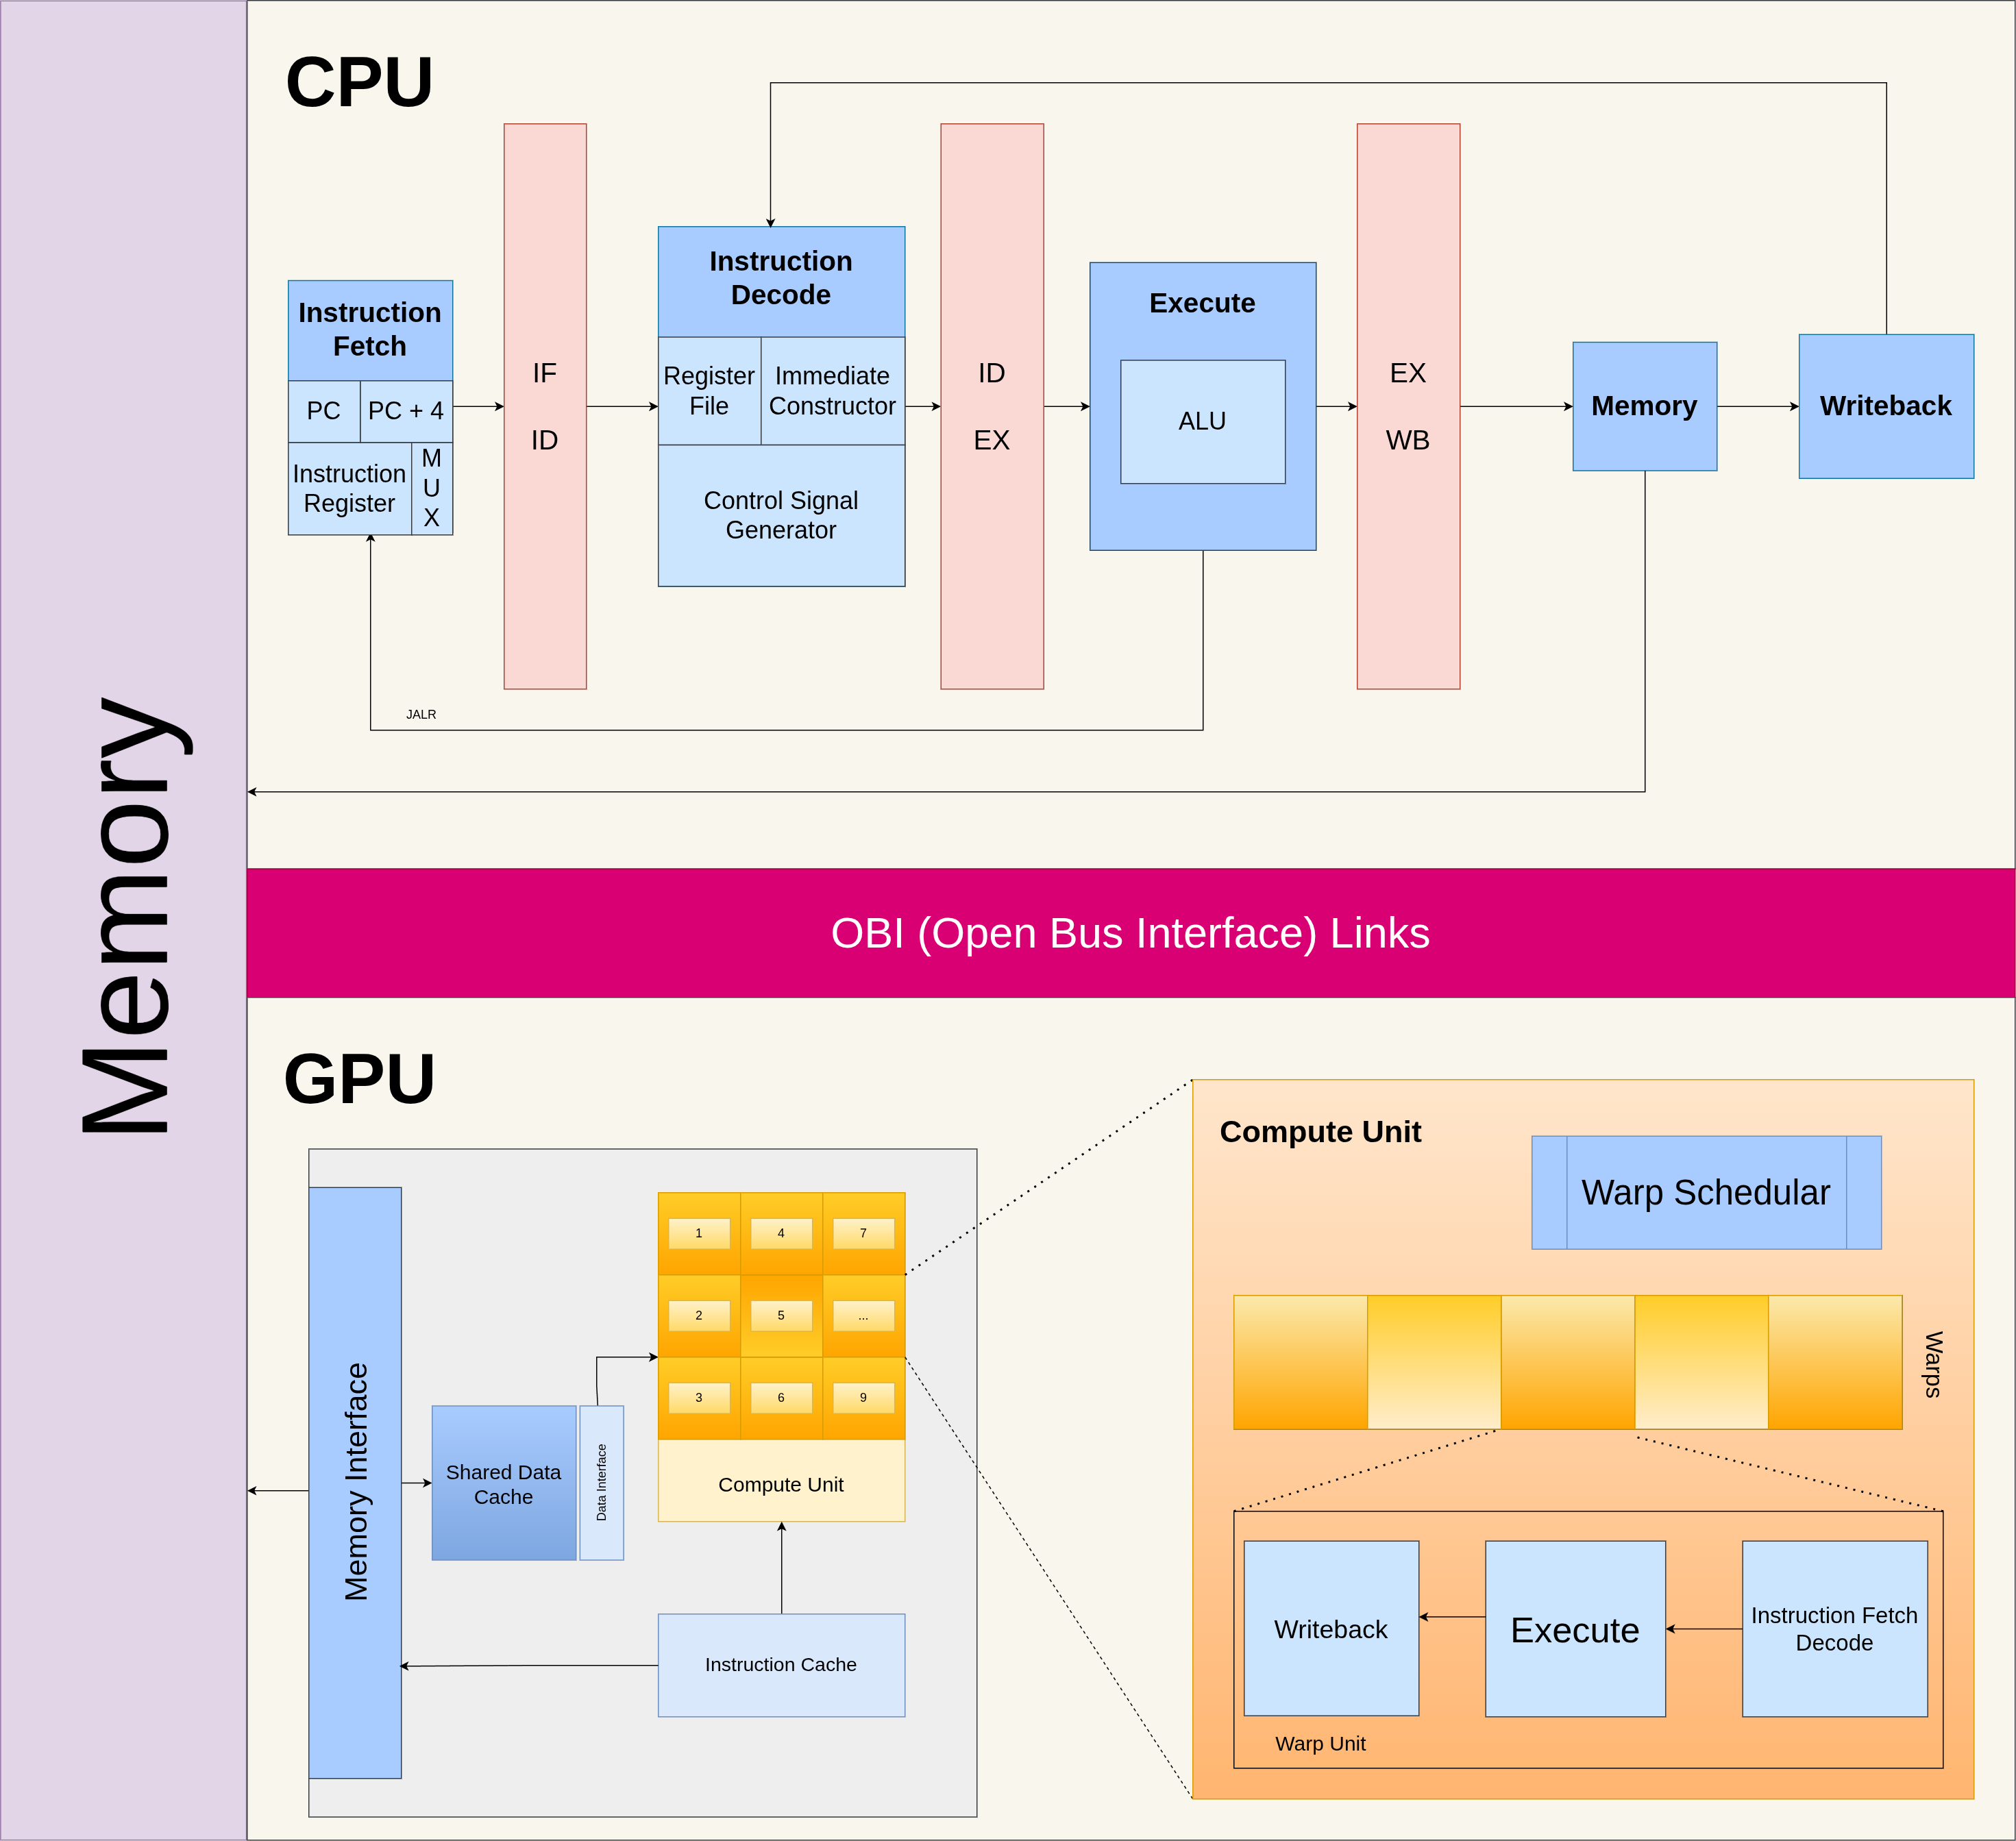
\includegraphics[width=1\textwidth]{pipeline_design.png}
        \caption{Simplified APU Pipeline Design}
        \label{fig.example}
\end{figure*}

The RISC-V-based APU architecture integrates CPU and GPU elements on a unified platform through a shared interconnect fabric, exemplified by the OpenBus Interface (OBI), which enables seamless communication between heterogeneous cores. As show in e-GPU, The system supports coherent memory sharing while balancing latency and bandwidth to sustain efficient task execution across compute units. The e-GPU operates as an independent accelerator with dedicated OBI master and slave ports for memory transactions and configuration, along with an interrupt line for real-time synchronization with the host. Power and clock gating mechanisms tied to the host power manager allow dynamic energy scaling, ensuring optimal performance and power efficiency for embedded and TinyAI-class workloads.

The host subsystem features a lightweight RISC-V processor optimized for control-intensive tasks and acts as the orchestration layer for the GPU, managing kernel dispatch, memory allocation, and execution flow through a high-bandwidth interconnect and low-latency SRAM banks. A minimalist runtime environment, built on Newlib and a compact OpenCL-like API, enables host–accelerator coordination without dependence on full operating systems or multithreading. This hardware-software co-design approach allows applications to be compiled into single executables with static resource definition, simplifying deployment and runtime management. FPGA-based validation of the system supports experimentation with ISA-level modifications, pipeline tuning, and memory hierarchies, providing a flexible framework for evaluating performance-power tradeoffs in processing environments.

\section{\uppercase{Conclusion}}
The RISC-V ecosystem has demonstrated significant progress towards realizing flexible and extensible processor designs suitable for a wide range of embedded and parallel computing applications. The foundational RV32I implementations continue to provide a robust baseline for efficient core processors, as shown by various FPGA-based single-cycle and pipelined architectures that balance throughput and implementation complexity effectively.

Recent advancements in heterogeneous RISC-V platforms, exemplified by projects such as Vortex and e-GPU, illustrate the practical integration of GPU-like acceleration into traditional CPUs to form APUs capable of exploiting data-parallel workloads across domains like AI, graphics, and edge computing. These designs highlight the feasibility of minimal ISA extensions, scalable multi-core configurations, and novel cache and memory hierarchies that maintain programmability via open-source toolchains and standardized interfaces.

The combined body of work emphasizes the importance of modularity, configurability, and hardware/software co-design in addressing evolving performance and application-specific requirements. Challenges remain in optimizing architectural complexity, synchronization, and communication across heterogeneous cores while ensuring energy-efficient operation suitable for resource-constrained environments. Overall, these efforts present an encouraging future trajectory for RISC-V APUs, promoting more versatile, open, and high-performance computing architectures tailored to contemporary embedded and parallel computation needs.

\begin{thebibliography}{99}

\bibitem{Rao2024}
Rao, M., Niranjan, P., \& MJ, D. K. (2024, October). Design and Implementation of 32-bit RISC-V Processor Using Verilog. In \textit{2024 IEEE International Conference on Distributed Computing, VLSI, Electrical Circuits and Robotics (DISCOVER)} (pp. 181-186). IEEE.

\bibitem{Tine2021}
Tine, B., Elsabbagh, F., Yalamarthy, K., \& Kim, H. (2021). Vortex: Extending the RISC-V ISA for GPGPU and 3D-Graphics Research. In \textit{54th Annual IEEE/ACM International Symposium on Microarchitecture (MICRO)} (pp. 1-13). ACM.

\bibitem{Machetti2025}
Machetti, S., Schiavone, P. D., Orlandic, L., Huang, D., Kasap, D., Ansaloni, G., \& Atienza, D. (2025). e-GPU: An Open-Source and Configurable RISC-V Graphic Processing Unit for TinyAI Applications. \textit{IEEE Transactions on Embedded Systems}.

\bibitem{Goh2024}
Goh, J. K., \& Uttraphan, C. (2024). An Enhanced UTHM RISC-V Processor Core Architecture Implemented on FPGA. \textit{Evolution in Electrical and Electronic Engineering, 5}(2), 32-41.

\bibitem{Rodrigues2019}
Rodrigues, J. F. M. (2019). \textit{Configurable RISC-V softcore processor for FPGA implementation} (Master's thesis, Instituto Superior Técnico).

\bibitem{Li2019}
Li, Z., Hu, W., \& Chen, S. (2019, August). Design and implementation of CNN custom processor based on RISC-V architecture. In \textit{2019 IEEE 21st International Conference on High Performance Computing and Communications; IEEE 17th International Conference on Smart City; IEEE 5th International Conference on Data Science and Systems (HPCC/SmartCity/DSS)} (pp. 1945-1950). IEEE.

\bibitem{Begum2023}
Begum, S., \& Kumar, T. (2023). FPGA-based Implementation of 32-bit RISC-V Processor. \textit{International Journal of Engineering Research and Technology}.

\bibitem{Zhou2020}
Zhou, Y., Jin, X., \& Xiang, T. (2020). RISC-V Graphics Rendering Instruction Set Extensions for Embedded Chips. In \textit{Proceedings of the 2020 ACM Symposium on Embedded Computing}. ACM.

\bibitem{Matthews2021}
Matthews, E. et al. (2021). Soft-Processor Parameterized RISC-V. \textit{IEEE Transactions on Computers}.

\bibitem{Pol2021}
Pol, L. (2021). Lightweight Open-Source RISC-V Processor for IoT. In \textit{Mobility, Sensing, and Networking Conference}.

\bibitem{Miyazaki2020}
Miyazaki, H., Kanamori, T., Islam, M. A., \& Kise, K. (2020). RVCoreP: An optimized RISC-V soft processor of five-stage pipelining. \textit{IEICE TRANSACTIONS on Information and Systems, 103}(12), 2494-2503.

\bibitem{Barriga2021}
Barriga, A. et al. (2021). Synthesis and Verification of RISC-V Cores. In \textit{International Symposium on Embedded Systems}.

\bibitem{Jo2023}
Jo, S. et al. (2023). Single Cycle RISC-V Core Implementation. \textit{International Journal of Engineering Research and Technology}.

\bibitem{Jinyu2022}
Jinyu, J. et al. (2022). Implementing RISC-V ISA on FPGA. \textit{International Journal of Advanced Engineering}.

\bibitem{Bhatia2019}
Bhatia, N., D'Souza, M., \& Chakrabarti, S. K. (2019, February). Formalizing GPU Instruction Set Architecture in Coq. In \textit{Proceedings of the 12th Innovations in Software Engineering Conference} (pp. 1-5).

\bibitem{Elsabbagh2020}
Elsabbagh, F., Tine, B., Roshan, P., Lyons, E., Kim, E., Shim, D. E., ... \& Lim, S. K. (2020). Vortex: opencl compatible risc-v gpgpu. \textit{arXiv preprint arXiv:2002.12151}.

\bibitem{AlKadi2016}
Al Kadi, M., Janssen, B., \& Huebner, M. (2016, February). FGPU: An SIMT-architecture for FPGAs. In \textit{Proceedings of the 2016 ACM/SIGDA International Symposium on Field-Programmable Gate Arrays} (pp. 254-263).

\bibitem{OpenHW2019}
OpenHW Group. (2019). \textit{OpenBus Interface (OBI) Specification}. Retrieved from \texttt{https://openhwgroup.org/specifications/}

\bibitem{VortexGit}
Vortex GPGPU. (n.d.). GitHub repository. Retrieved from \texttt{https://github.com/vortexgpgpu/vortex}

\bibitem{SmolGPUGit}
Smol GPU. (n.d.). GitHub repository. Retrieved from \texttt{https://github.com/Grubre/smol-gpu}

\bibitem{RiscyGit}
RISCY. (n.d.). GitHub repository. Retrieved from \texttt{https://github.com/mongrelgem/RISCY}

\bibitem{RV32ISpec}
RISC-V Foundation. (2019). *The RISC-V Instruction Set Manual, Volume I: Unprivileged ISA, Version 2.1 (RV32I/64I/128I)*. Retrieved from \texttt{https://riscv.org/technical/specifications/}

\end{thebibliography}

\end{document}


